\section{Further contemporary RL algorithms}


%%%%%%%%%%%%%%%%%%%%%%%%%%%%%%%%%%%%%%%%%%%%%%%%%%%%%%%%%%%%%%%%%%
\subsection{Trust region policy optimization (TRPO)} 
%%%%%%%%%%%%%%%%%%%%%%%%%%%%%%%%%%%%%%%%%%%%%%%%%%%%%%%%%%%%%%%%%%

%%%%%%%%%%%%%%%%%%%%%%%%%%%%%%%%%%%%%%%%%%%%%%%%%%%%%%%%%%%%%
%% Reinterpreting the Policy Gradient for Stochastic Policies (1)%%
%%%%%%%%%%%%%%%%%%%%%%%%%%%%%%%%%%%%%%%%%%%%%%%%%%%%%%%%%%%%%
\setcounter{footnote}{0}
\frame{\frametitle{Reinterpreting the stochastic policy gradient (1)}
\vspace{-0.2cm}
\begin{itemize}
	\item In the following we will \hl{focus on stochastic policies} $\pi(\bm{u}|\bm{x})$ .\pause
	\item First, we rewrite the performance metric \eqref{eq:performance_metric_episodic} to obtain
		\begin{equation}
		J_{\pi} =\El{\sum_{k=0}^\infty \gamma^k R_k}{\pi}.
	\end{equation}\vspace{-0.5cm}\pause
	\item Using the advantage $a_\pi(\bm{x},\bm{u})= q_{\pi}(\bm{x},\bm{u})-v_{\pi}(\bm{x})$ we can calculate the performance of an updated policy $\bm{\pi}\rightarrow\tilde{\bm{\pi}}$\footnote{proof from: S. Kakade and J. Langford, \textit{Approximately optimal approximate reinforcement learning}, ICML, vol. 2, pp 267-274, 2002}:
		\begin{equation}
		\label{eq:TRPO_perf_change}
		J_{\tilde{\pi}} =J_{\pi} + \int_\mathcal{X}p^{\tilde{\pi}}(\bm{x})\int_{\mathcal{U}} \tilde{\pi}(\bm{u}|\bm{x})a_\pi(\bm{x},\bm{u}).
	\end{equation}\vspace{-0.5cm}\pause
	\item While for finite MDPs, the policy improvement theorem guaranteed  $J_{\tilde{\pi}} \geq J_{\pi}$ for each policy update, there might be some states where $\int_{\mathcal{U}} \tilde{\pi}(\bm{u}|\bm{x})a_\pi<0$ for continuous MDPs using function approximation. 
\end{itemize}
}

%%%%%%%%%%%%%%%%%%%%%%%%%%%%%%%%%%%%%%%%%%%%%%%%%%%%%%%%%%%%%
%% Reinterpreting the Policy Gradient for Stochastic Policies (2)%%
%%%%%%%%%%%%%%%%%%%%%%%%%%%%%%%%%%%%%%%%%%%%%%%%%%%%%%%%%%%%%
\frame{\frametitle{Reinterpreting the stochastic policy gradient  (2)}
\begin{itemize}
	\item For easier calculation, we introduce a local approximation to \eqref{eq:TRPO_perf_change}
	\begin{equation}
		\mathcal{L}_{\pi}(\tilde{\pi}) =J_{\pi} + \int_\mathcal{X}p^{\pi}(\bm{x})\int_{\mathcal{U}} \tilde{\pi}(\bm{u}|\bm{x})a_\pi(\bm{x},\bm{u})
	\end{equation}
	where $p^{\pi}(\bm{x})$ is used instead of $p^{\tilde{\pi}}(\bm{x})$, i.e., neglecting the state distribution change due to a policy update.\pause
	\item For any parametrized and differentiable policy $\pi_{\bm{\theta}}(\bm{u}|\bm{x})$, it can be shown that
	\begin{equation}
	\begin{split}
		 \mathcal{L}(\pi_{\bm{\theta}_0}) &= J(\pi_{\bm{\theta}_0}),\\
		\nabla_{\bm{\theta}}\mathcal{L}_{\pi_{\bm{\theta}_0}}(\pi_{\bm{\theta}})|_{\bm{\theta}=\bm{\theta}_0} &= \nabla_{\bm{\theta}}J(\pi_{\bm{\theta}})|_{\bm{\theta}=\bm{\theta}_0}
	\end{split}	
	\end{equation}
	for any initial parameter set $\bm{\theta}_0$.\pause
	 \item For a sufficiently small step size, improving $\mathcal{L}_{\pi_{\bm{\theta}_0}}$ will also improve $J$. \pause
\end{itemize}
\begin{block}{}
However, we do not know how much the actual stochastic policy will change while moving through the parameter space. Hence, we do not have a good decision basis to choose the policy gradient step size.   
\end{block}
}

%%%%%%%%%%%%%%%%%%%%%%%%%%%%%%%%%%%%%%%%%%%%%%%%%%%%%%%%%%%%%
%% Adding a Trust Region Constraint (1)%%
%%%%%%%%%%%%%%%%%%%%%%%%%%%%%%%%%%%%%%%%%%%%%%%%%%%%%%%%%%%%%
\frame{\frametitle{Adding a trust region constraint (1)}
\begin{itemize}
	\item From the previous discussion it can be concluded that we want a \hl{metric describing how much a policy is changed in the action space when updating the policy in the parameter space}. \pause 
	\item Against this background, we make use of the \hl{Kullback-Leibler divergence} (also called relative entropy)
	\begin{equation}
		D_{\mathrm{KL}}(P \parallel Q) = \int_{-\infty}^\infty p(x) \log\left(\frac{p(x)}{q(x)}\right)\, \mathrm{d}x
	\end{equation}
	defined for continuous distributions $P$ and $Q$ with their probability densities $p$ and $q$. \pause
	\item Example: for two multivariate Gaussian distributions of equal dimensions $d$, with means $\bm{\mu}_0, \bm{\mu}_1$ and with (non-singular) covariance matrix $\bm{\Sigma}_0, \bm{\Sigma}_1$ we receive
\end{itemize}
	\small
	\begin{align*}
D_{\mathrm{KL}}\left(\mathcal{N}_0 \parallel \mathcal{N}_1\right) =  \frac{1}{2}&\left(\mathrm{tr}\left(\bm{\Sigma}_1^{-1}\bm{\Sigma}_0\right) + \left(\bm{\mu}_1 - \bm{\mu}_0\right)\T \bm{\Sigma}_1^{-1}\left(\bm{\mu}_1 - \bm{\mu}_0\right) \right. \\ &\left.- d + \ln\left(\frac{\det\bm{\Sigma}_1}{\det\bm{\Sigma}_0}\right) \right).		
	\end{align*}
	\normalsize
}

%%%%%%%%%%%%%%%%%%%%%%%%%%%%%%%%%%%%%%%%%%%%%%%%%%%%%%%%%%%%%
%% Adding a Trust Region Constraint (2)%%
%%%%%%%%%%%%%%%%%%%%%%%%%%%%%%%%%%%%%%%%%%%%%%%%%%%%%%%%%%%%%
\frame{\frametitle{Adding a trust region constraint (2)}
\begin{itemize}
	\item The \hl{trust region policy optimization (TRPO)} updates the policy parameters while constraining the KL divergence between the new and the old policy distribution:
	\begin{equation}
	\label{eq:TRPO_opt_prob}
	\begin{split}
		 &\max_{\bm{\theta}}  \, \mathcal{L}_{\bm{\theta}_k}(\bm{\theta}),\\
		 \mbox{s.t.} \quad\quad  & \overline{D}_{\mathrm{KL}}(\bm{\theta}_k, \bm{\theta})\leq\kappa
	\end{split}
	\end{equation}\pause
	with 
\end{itemize}
\vspace{0.15cm}
	\begin{equation*}
\overline{D}_{\mathrm{KL}}(\bm{\theta}_k, \bm{\theta})=\overline{D}_{\mathrm{KL}}(\pi_{\bm{\theta}_k}, \pi_{\bm{\theta}})=\El{D_{\mathrm{KL}}(\pi_{\bm{\theta}_k}(\cdot|\bm{X}) \parallel \pi_{\bm{\theta}}(\cdot|\bm{X}))}{\pi_{\bm{\theta}_k}}.
	\end{equation*}
	\vspace{-0.25cm}\pause
\begin{itemize}
	\item Hence, we want to \hl{limit the average KL divergence w.r.t. the states visited by the old policy}.\pause
	\item The constraint $\kappa$ is a TRPO hyperparameter (typically $\kappa<<1$). \pause
	\item Although \eqref{eq:TRPO_opt_prob}  does not provide any formal convergence guarantee, we at least have a link between changes in the parameter and policy distribution space. Therefore, \hl{we can use this tool to prevent erratic policy changes}.  
\end{itemize}
}

%%%%%%%%%%%%%%%%%%%%%%%%%%%%%%%%%%%%%%%%%%%%%%%%%%%%%%%%%%%%%
%% Smooth Policy Updates via TRPO %%
%%%%%%%%%%%%%%%%%%%%%%%%%%%%%%%%%%%%%%%%%%%%%%%%%%%%%%%%%%%%%
\frame{\frametitle{Smooth policy updates via TRPO}
\begin{figure}
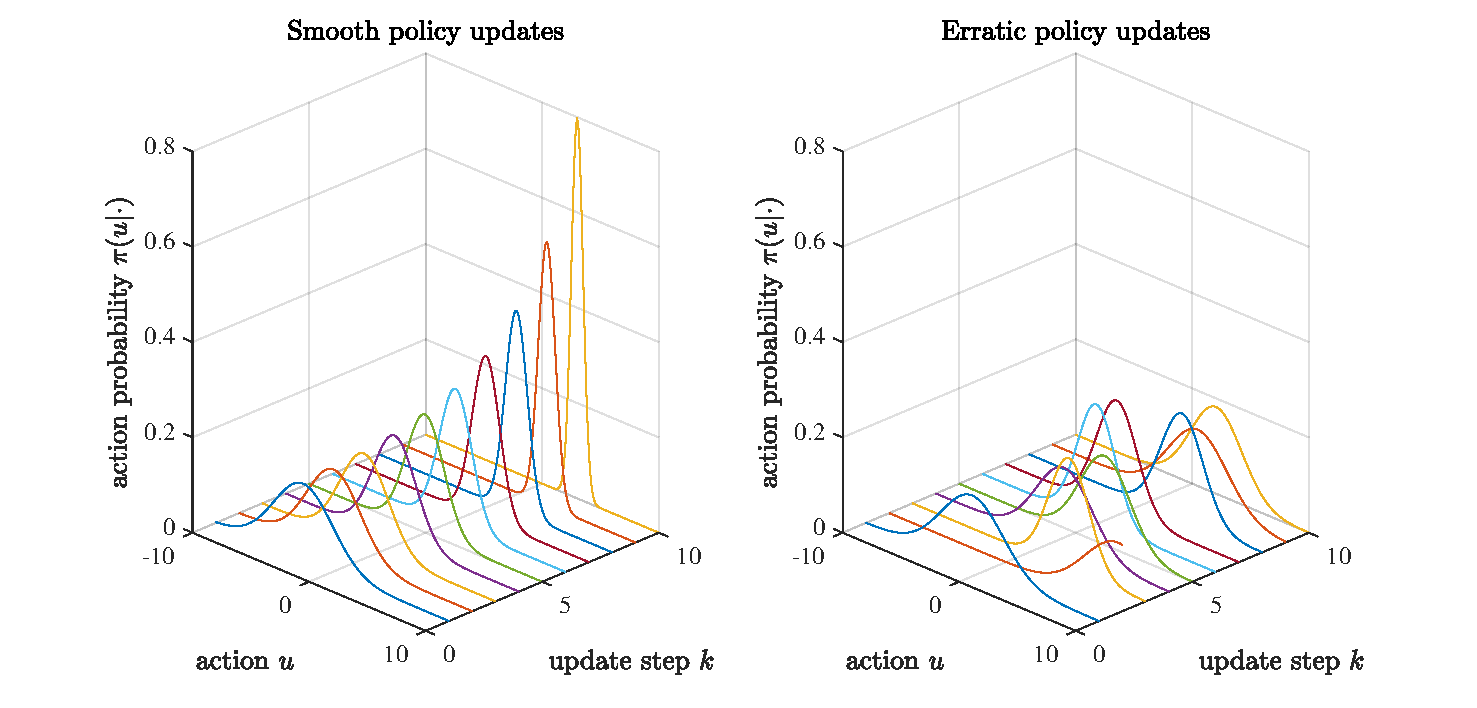
\includegraphics[height=5.75cm]{fig/lec13/TRPO_Style_Updates.pdf}
\caption{Simplified representation of the policy evolution for a scalar action given some fixed state. Left: TRPO-style updates finding the optimal action with increasing probability. Right: Unmonitored policy distributions not converging towards an optimal policy ('policy chattering').}
\label{fig:TRPO_Style_Updates}
\end{figure}
}	

%%%%%%%%%%%%%%%%%%%%%%%%%%%%%%%%%%%%%%%%%%%%%%%%%%%%%%%%%%%%%
%% Sample-Based Estimation of the Objective and Constraint%%
%%%%%%%%%%%%%%%%%%%%%%%%%%%%%%%%%%%%%%%%%%%%%%%%%%%%%%%%%%%%%
\frame{\frametitle{Sample-based objective and constraint estimation (1)}
\begin{itemize}
	\item To actually solve \eqref{eq:TRPO_opt_prob} we will make use of samplings from \hl{Monte Carlo rollouts}.\pause
	\item Expanding the objective yields
	\begin{equation}
		\max_{\bm{\theta}}  \, \mathcal{L}_{\bm{\theta}_k}(\bm{\theta})= \max_{\bm{\theta}} \, J_{\pi_k} + \int_\mathcal{X}p^{\pi_k}(\bm{x})\int_{\mathcal{U}} \pi_{\bm{\theta}}(\bm{u}|\bm{x})a_{\pi_k}(\bm{x},\bm{u}).
	\end{equation}\pause
	\item The first term $J_{\pi_k}$ can be dropped, since it is irrelevant for the optimization result (constant).\pause
	\item Using samples we can approximate $\int_\mathcal{X}p^{\pi_k}(\bm{x})\approx\frac{1}{1-\gamma}\El{\bm{X}}{\pi_{\bm{\theta}_k}}$.\pause
	\item Moreover, $\int_{\mathcal{U}} \pi_{\bm{\theta}}(\bm{u}|\bm{x})a_{\pi_k}(\bm{x},\bm{u})\approx\El{\frac{\pi_{\bm{\theta}}(\bm{U}|\bm{X})}{\pi_{\bm{\theta}_k}(\bm{U}|\bm{X})}a_{\pi_k}(\bm{X},\bm{U})}{\pi_{\bm{\theta}_k}}$ is also approximated applying importance sampling based on data from the old policy.\pause
	\item Hence, the sampled objective is
	\begin{equation}
		\max_{\bm{\theta}} \,\El{\frac{\pi_{\bm{\theta}}(\bm{U}|\bm{X})}{\pi_{\bm{\theta}_k}(\bm{U}|\bm{X})}a_{\pi_k}(\bm{X},\bm{U})}{\pi_{\bm{\theta}_k}}.
	\end{equation}
\end{itemize}
}

%%%%%%%%%%%%%%%%%%%%%%%%%%%%%%%%%%%%%%%%%%%%%%%%%%%%%%%%%%%%%
%% Sample-Based Estimation of the Objective and Constraint%%
%%%%%%%%%%%%%%%%%%%%%%%%%%%%%%%%%%%%%%%%%%%%%%%%%%%%%%%%%%%%%
\frame{\frametitle{Sample-based objective and constraint estimation (2)}
\begin{itemize}
	\item Applying the previous sample-based estimation we obtain
\end{itemize}
\vspace{0.15cm}
		\begin{equation}
	\label{eq:TRPO_opt_prob_sample}
	\begin{split}
		 &\bm{\theta}_{k+1} = \argmax_{\bm{\theta}} \,\El{\frac{\pi_{\bm{\theta}}(\bm{U}|\bm{X})}{\pi_{\bm{\theta}_k}(\bm{U}|\bm{X})}a_{\pi_k}(\bm{X},\bm{U})}{\pi_{\bm{\theta}_k}},\\
		 \mbox{s.t.} \quad\quad  & \El{D_{\mathrm{KL}}(\pi_{\bm{\theta}_k}(\cdot|\bm{X}) \parallel \pi_{\bm{\theta}}(\cdot|\bm{X}))}{{\pi_{\bm{\theta}_k}}}\leq\kappa.
	\end{split}
	\end{equation}
	\vspace{-0.25cm}
\begin{itemize}\pause
	\item Hence, we have a \hl{three-step procedure} for each TRPO update:\pause
\end{itemize}
\begin{enumerate}
	\item Use Monte Carlo simulations based on the old policy to obtain data.\pause
	\item Use the data to construct \eqref{eq:TRPO_opt_prob_sample}.\pause
	\item Solve the constrained optimization problem to update the policy parameter vector. 
\end{enumerate}\pause
\begin{block}{}
Solving  \eqref{eq:TRPO_opt_prob_sample} is generally a nonlinear optimization problem. The original TRPO implementation uses a local objective and constraint approximation together with conjugate gradient and line search algorithms. However, many other constrained-nonlinear solvers are also applicable.
\end{block}
}

%%%%%%%%%%%%%%%%%%%%%%%%%%%%%%%%%%%%%%%%%%%%%%%%%%%%%%%%%%%%%
%% Generalized Advantage Estimation %%
%%%%%%%%%%%%%%%%%%%%%%%%%%%%%%%%%%%%%%%%%%%%%%%%%%%%%%%%%%%%%
\frame{\frametitle{Generalized advantage estimation}
\setcounter{footnote}{0}
\begin{itemize}
	\item Having data $\left\langle \bm{x}, \bm{u}, r, \bm{x}'\right\rangle$ in $\bm{\mathcal{D}}$ from a Monte Carlo rollout available, an imporant problem is to estimate $a_{\pi_k}(\bm{x},\bm{u})$ in \eqref{eq:TRPO_opt_prob_sample}.\pause
	\item A particular suggestion in the TRPO context is to use a \hl{generalized advantage estimator (GAE)} \footnote{cf. J. Schulmann et al., \textit{High Dimensional Continuous Control Using Generalized Advantage Estimation}, \href{https://arxiv.org/abs/1506.02438}{https://arxiv.org/abs/1506.02438}, 2015} defined as
	\begin{equation}
	\label{eq:GAE}
		\hat{a}_k^{(\gamma, \lambda)} = \sum_{i=0}^\infty (\gamma\lambda)^i\delta_{k+i}.
	\end{equation}\pause
	\item Here, $\delta_{k}=r_k+\gamma v(\bm{x}_{k+1})-v(\bm{x}_{k})$ is a single advantage sample.\pause
	\item Hence, the GAE is the exponentially-weighted average of the discounted advantage samples with an additional weighting $\lambda$.\pause
	\item Similar formulation compared to TD$(\lambda)$ but the estimator's target is the advantage. \pause
	\item The choice of $(\gamma\lambda)$ trade-offs the bias and variance of the estimator. 
\end{itemize}	
}

%%%%%%%%%%%%%%%%%%%%%%%%%%%%%%%%%%%%%%%%%%%%%%%%%%%%%%%%%%%%%
%% Summary %%
%%%%%%%%%%%%%%%%%%%%%%%%%%%%%%%%%%%%%%%%%%%%%%%%%%%%%%%%%%%%%
\frame{\frametitle{TRPO summary}
\vspace{-0.1cm}
The TRPO's key facts are:
\begin{itemize}
	\item The TRPO constrains policy distribution changes when updating the policy parameters (for stochastic policies and on-policy learning).\pause
	\item The objective is to enable a monotonically improving learning process.\pause
	\item Using trust regions, erratic policy updates should be prevented.\pause
\end{itemize}	
The TRPO's main hurdles are:
\begin{itemize}
	\item Constructing the objective function and constraint requires Monte Carlo rollouts (time consuming, data inefficient).\pause
	\item When the sampled optimization problem is set up, a nonlinear and constrained optimization step is required (no simple policy gradient, computational costly).\pause
\end{itemize}\pause	
\begin{block}{}
We will not provide any specific TRPO implementation suggestion at this point, since this is rather cumbersome. Instead we will move forward to a similar algorithm which is pursuing the same goal (prevent erratic policy changes) with a much simpler implementation.  
\end{block}
}

%%%%%%%%%%%%%%%%%%%%%%%%%%%%%%%%%%%%%%%%%%%%%%%%%%%%%%%%%%%%%%%%%%
\subsection{Proximal policy optimization (PPO)} 
%%%%%%%%%%%%%%%%%%%%%%%%%%%%%%%%%%%%%%%%%%%%%%%%%%%%%%%%%%%%%%%%%%


%%%%%%%%%%%%%%%%%%%%%%%%%%%%%%%%%%%%%%%%%%%%%%%%%%%%%%%%%%%%%
%% Background and Motivation %%
%%%%%%%%%%%%%%%%%%%%%%%%%%%%%%%%%%%%%%%%%%%%%%%%%%%%%%%%%%%%%
\frame{\frametitle{Background and motivation}
\begin{itemize}
	\item The upcoming \hl{proximal policy optimization (PPO)} algorithm tries to mimic the constrained TRPO problem
\end{itemize}	
\vspace{0.15cm}
		\begin{equation*}
	\begin{split}
		 &\bm{\theta}_{k+1} = \argmax_{\bm{\theta}} \,\El{\frac{\pi_{\bm{\theta}}(\bm{U}|\bm{X})}{\pi_{\bm{\theta}_k}(\bm{U}|\bm{X})}a_{\pi_k}(\bm{X},\bm{U})}{\pi_{\bm{\theta}_k}},\\
		 \mbox{s.t.} \quad\quad  & \El{D_{\mathrm{KL}}(\pi_{\bm{\theta}_k}(\cdot|\bm{X}) \parallel \pi_{\bm{\theta}}(\cdot|\bm{X}))}{{\pi_{\bm{\theta}_k}}}\leq\kappa.
	\end{split}
	\end{equation*}
based on related unconstrained problems. 
\pause
\begin{itemize}
	\item Hence, the objective will be reformulated to incorporate mechanisms preventing excessively large variations of the policy distribution during a parameter update (leading to an updated policy with sufficient proximity to the old one).  \pause
	\item Moreover, \hl{PPO incorporates two variants} which we will discuss:
	\begin{enumerate}
	\item Clipping the surrogate objective,\pause
	\item Adaptive tuning of a KL-associated penalty coefficient.
\end{enumerate}
\end{itemize}
}

%%%%%%%%%%%%%%%%%%%%%%%%%%%%%%%%%%%%%%%%%%%%%%%%%%%%%%%%%%%%%
%% Clipped Surrogate Objective %%
%%%%%%%%%%%%%%%%%%%%%%%%%%%%%%%%%%%%%%%%%%%%%%%%%%%%%%%%%%%%%
\frame{\frametitle{Clipped surrogate objective}
\begin{itemize}
	\item The first approach is based on the following \hl{clipped objective}:
\end{itemize}
\vspace{0.25cm}
\small
\begin{equation}
\label{eq:PPO_CSO}
		\hspace{-0.2cm}\El{\min\left\{\frac{\pi_{\bm{\theta}}(\bm{U}|\bm{X})}{\pi_{\bm{\theta}_k}(\bm{U}|\bm{X})}a_{\pi_k}(\bm{X},\bm{U}), \mathrm{clip}\left(\frac{\pi_{\bm{\theta}}(\bm{U}|\bm{X})}{\pi_{\bm{\theta}_k}(\bm{U}|\bm{X})}, 1-\epsilon, 1+\epsilon\right)a_{\pi_k}(\bm{X},\bm{U})\right\}}{\pi_{\bm{\theta}_k}}.
\end{equation}\pause
\normalsize
\begin{itemize}
	\item Above, $\epsilon<1$ is a PPO hyperparameter serving as a regularizer.\pause
	\item The first element of $\min\{\cdot\}$ is the previous TPRO objective.\pause
	\item The second element of $\min\{\cdot\}$ modifies the surrogate objective by clipping the importance sampling ratio $\pi_{\bm{\theta}}/\pi_{\bm{\theta}_k}$.\pause
	\item The latter should remove the incentive for moving the importance sampling ratio outside of the interval $[1-\epsilon, 1+\epsilon]$.\pause
	\item The modified objective is therefore a lower bound of the unclipped TRPO objective. 
\end{itemize}
}

%%%%%%%%%%%%%%%%%%%%%%%%%%%%%%%%%%%%%%%%%%%%%%%%%%%%%%%%%%%%%
%% Clipped Surrogate Objective: Positive Advantage %%
%%%%%%%%%%%%%%%%%%%%%%%%%%%%%%%%%%%%%%%%%%%%%%%%%%%%%%%%%%%%%
\frame{\frametitle{Clipped surrogate objective: positive advantage}
\begin{itemize}
	\item Consider a single sample $(\bm{x}, \bm{u})$ with a \hl{positive advantage} $a_{\pi_k}(\bm{x},\bm{u})$:\pause
\end{itemize}
\vspace{0.1cm}
\begin{equation*}
		\max_{\bm{\theta}}\,\min\left\{\frac{\pi_{\bm{\theta}}(\bm{u}|\bm{x})}{\pi_{\bm{\theta}_k}(\bm{u}|\bm{x})}a_{\pi_k}(\bm{x},\bm{u}), \mathrm{clip}\left(\frac{\pi_{\bm{\theta}}(\bm{u}|\bm{x})}{\pi_{\bm{\theta}_k}(\bm{u}|\bm{x})}, 1-\epsilon, 1+\epsilon\right)a_{\pi_k}(\bm{x}, \bm{u})\right\}.
\end{equation*}\pause
\begin{itemize}
	\item Because the advantage is positive, the objective will increase if the action becomes more likely, i.e., if $\pi_{\bm{\theta}}(\bm{u}|\bm{x})$ increases.\pause
	\item If $\pi_{\bm{\theta}}(\bm{u}|\bm{x}) > (1+\epsilon)\pi_{\bm{\theta}_k}(\bm{u}|\bm{x})$ the clipping becomes active.\pause
	\item Hence, the objective reduces to
	\begin{equation*}
		\max_{\bm{\theta}}\,\min\left\{\frac{\pi_{\bm{\theta}}(\bm{u}|\bm{x})}{\pi_{\bm{\theta}_k}(\bm{u}|\bm{x})},  1+\epsilon\right\}a_{\pi_k}(\bm{x},\bm{u}).
\end{equation*}\pause
	\item Due to the $\min\{\cdot\}$ operator, the entire objective is therefore limited to $(1+\epsilon)a_{\pi_k}(\bm{x},\bm{u})$.\pause
	\item Interpretation: the new policy does not benefit from going very away from the old policy distribution.
\end{itemize}
}

%%%%%%%%%%%%%%%%%%%%%%%%%%%%%%%%%%%%%%%%%%%%%%%%%%%%%%%%%%%%%
%% Clipped Surrogate Objective: Negative Advantage %%
%%%%%%%%%%%%%%%%%%%%%%%%%%%%%%%%%%%%%%%%%%%%%%%%%%%%%%%%%%%%%
\frame{\frametitle{Clipped surrogate objective: negative advantage}
\begin{itemize}
	\item Consider a single sample $(\bm{x}, \bm{u})$ with a \hl{negative advantage} $a_{\pi_k}(\bm{x},\bm{u})$:\pause
\end{itemize}
\vspace{0.1cm}
\begin{equation*}
		\max_{\bm{\theta}}\,\min\left\{\frac{\pi_{\bm{\theta}}(\bm{u}|\bm{x})}{\pi_{\bm{\theta}_k}(\bm{u}|\bm{x})}a_{\pi_k}(\bm{x},\bm{u}), \mathrm{clip}\left(\frac{\pi_{\bm{\theta}}(\bm{u}|\bm{x})}{\pi_{\bm{\theta}_k}(\bm{u}|\bm{x})}, 1-\epsilon, 1+\epsilon\right)a_{\pi_k}(\bm{x},\bm{u})\right\}.
\end{equation*}\pause
\begin{itemize}
	\item Because the advantage is negative, the objective will increase if the action becomes less likely, i.e., if $\pi_{\bm{\theta}}(\bm{u}|\bm{x})$ decreases.\pause
	\item If $\pi_{\bm{\theta}}(\bm{u}|\bm{x}) < (1-\epsilon)\pi_{\bm{\theta}_k}(\bm{u}|\bm{x})$ the clipping becomes active.\pause
	\item Hence, the objective reduces to
	\begin{equation*}
		\max_{\bm{\theta}}\,\max\left\{\frac{\pi_{\bm{\theta}}(\bm{u}|\bm{x})}{\pi_{\bm{\theta}_k}(\bm{u}|\bm{x})},  1-\epsilon\right\}a_{\pi_k}(\bm{x},\bm{u}).
\end{equation*}\pause
	\item Due to the $\max\{\cdot\}$ operator, the entire objective is limited to $(1-\epsilon)a_{\pi_k}(\bm{x},\bm{u})$.\pause
\end{itemize}
}

%%%%%%%%%%%%%%%%%%%%%%%%%%%%%%%%%%%%%%%%%%%%%%%%%%%%%%%%%%%%%
%% Adaptive KL Penalty %%
%%%%%%%%%%%%%%%%%%%%%%%%%%%%%%%%%%%%%%%%%%%%%%%%%%%%%%%%%%%%%
\frame{\frametitle{Adaptive KL penalty}
\begin{itemize}
	\item The second PPO variant makes use of the following \hl{KL-penalized objective}
\end{itemize}
\vspace{0.15cm}
\small
	\begin{equation}
	\label{eq:PPO_AKP}
      \El{\frac{\pi_{\bm{\theta}}(\bm{U}|\bm{X})}{\pi_{\bm{\theta}_k}(\bm{U}|\bm{X})}a_{\pi_k}(\bm{X},\bm{U})\hl{-\beta D_{\mathrm{KL}}(\pi_{\bm{\theta}_k}(\cdot|\bm{X}) \parallel \pi_{\bm{\theta}}(\cdot|\bm{X}))}}{\pi_{\bm{\theta}_k}}.		
	\end{equation}
	\normalsize\pause
	\vspace{-0.25cm}
\begin{itemize}
	\item Transfers the KL-based constraint into a penalty for large policy distribution changes.\pause
	\item The parameter $\beta$ weights the penalty against the policy improvement.\pause
	\item The original PPO implementation suggests an adaptive tuning of $\beta$ w.r.t. the sampled average KL divergence $\overline{D}_{\mathrm{KL}}(\bm{\theta}_k, \bm{\theta})$ estimated from previous experience
	\begin{equation}
	\begin{split}
		  \overline{D}_{\mathrm{KL}}(\bm{\theta}_k, \bm{\theta}) < \overline{D}^*_{\mathrm{KL}}: &\quad \beta \leftarrow \beta/2,\\ 
			\overline{D}_{\mathrm{KL}}(\bm{\theta}_k, \bm{\theta}) > \overline{D}^*_{\mathrm{KL}}: &\quad \beta \leftarrow \beta \cdot 2.
	\end{split}	
	\end{equation}
	with some target value of the KL divergence $\overline{D}^*_{\mathrm{KL}}$ (additional hyperparameter). 
\end{itemize}
}

%%%%%%%%%%%%%%%%%%%%%%%%%%%%%%%%%%%%%%%%%%%%%%%%%%%%%%%%%%%%%
%% Algorithmic Implementation: PPO %%
%%%%%%%%%%%%%%%%%%%%%%%%%%%%%%%%%%%%%%%%%%%%%%%%%%%%%%%%%%%%%
\frame{\frametitle{Algo. implementation: PPO}
\setlength{\algomargin}{0.5em}
\begin{algorithm}[H]
\small
\SetKwInput{Input}{input} 
\SetKwInput{Output}{output}
\SetKwInput{Init}{init}
\SetKwInput{Param}{parameter}
\Input{diff. stochastic policy fct. $\pi(\bm{u}|\bm{x},\bm{\theta})$ and value fct. $\hat{v}(\bm{x},\bm{w})$}
\Param{step sizes $\{\alpha_{w}, \alpha_{\theta}\}\in\left\{\mathbb{R}|0<\alpha\right\}$}
\Init{weights $\bm{w}\in\mathbb{R}^{\zeta}$ and $\bm{\theta}\in\mathbb{R}^d$ arbitrarily, memory $\bm{\mathcal{D}}$}\pause
 \For{$j=1,2,\ldots,$ (sub-)episodes}{
		initialize $\bm{x}_0$ (if new episode)\; 
		collect a set of tuples $\left\langle \bm{x}_k, \bm{u}_k, r_{k+1}, \bm{x}_{k+1}\right\rangle$ by a rollout using $\pi(\bm{u}|\bm{x},\bm{\theta}_j)$\;\pause
		store them in $\bm{\mathcal{D}}$\;\pause
		estimate the advantage $\hat{a}_{\pi_j}(\bm{x},\bm{u})$ based on $\hat{v}(\bm{x},\bm{w}_j)$ and $\bm{\mathcal{D}}$ (e.g., GAE)\;\pause
		$\bm{\theta}_{j+1}\leftarrow$ policy gradient update based on the PPO variant \eqref{eq:PPO_CSO} or \eqref{eq:PPO_AKP}\;\pause
		$\bm{w}_{j+1}\leftarrow$ minimizing the mean-squared TD errors using $\bm{\mathcal{D}}$ (critic)\;\pause
		delete entries in $\bm{\mathcal{D}}$ (due to on-policy learning)\;
	}
\caption{Proximal policy optimization (output: parameter vectors $\bm{\theta}^*$ for $\pi^*(\bm{u}|\bm{x},\bm{\theta}^*)$ and $\bm{w}^*$ for $\hat{v}^*(\bm{x}, \bm{w}^*))$}
\label{algo:PPO}
\end{algorithm}
}

%%%%%%%%%%%%%%%%%%%%%%%%%%%%%%%%%%%%%%%%%%%%%%%%%%%%%%%%%%%%%
%% Some PPO Remarks %%
%%%%%%%%%%%%%%%%%%%%%%%%%%%%%%%%%%%%%%%%%%%%%%%%%%%%%%%%%%%%%
\frame{\frametitle{Some PPO remarks}
\setcounter{footnote}{0}
\begin{itemize}
	\item Clipping the surrogate objective \eqref{eq:PPO_CSO} was reported to achieve higher performances than the KL penalty \eqref{eq:PPO_AKP}.\footnote{cf. original PPO paper results by J. Schulman et al., \textit{Proximal Policy Optimization Algorithms}, \href{https://arxiv.org/abs/1707.06347}{https://arxiv.org/abs/1707.06347}, 2017}\pause
	\item Like TRPO, PPO is an on-policy algorithm. Hence, the memory $\bm{\mathcal{D}}$ is not a rolling replay buffer (cf. off-policy algorithms like DQN, DDPG or TD3) but a \hl{rollout buffer} using one fixed policy.\pause
	\item These rollouts are likely to result in an increased sample demand either using a simulator or a real experiment.\pause
\end{itemize}
\begin{block}{}
Although PPO is derived from a TRPO background pursuing monotonically increasing policy performance, its realization is based on multiple heuristics and approximations. Hence, there is no guarantee on achieving this goal and the specific performance of the PPO algorithm must be evaluated empirically given a certain application.  
\end{block}
}

%%%%%%%%%%%%%%%%%%%%%%%%%%%%%%%%%%%%%%%%%%%%%%%%%%%%%%%%%%%%%
%% Exemplary Performance Comparison %%
%%%%%%%%%%%%%%%%%%%%%%%%%%%%%%%%%%%%%%%%%%%%%%%%%%%%%%%%%%%%%
\frame{\frametitle{Exemplary performance comparison}
\begin{figure}
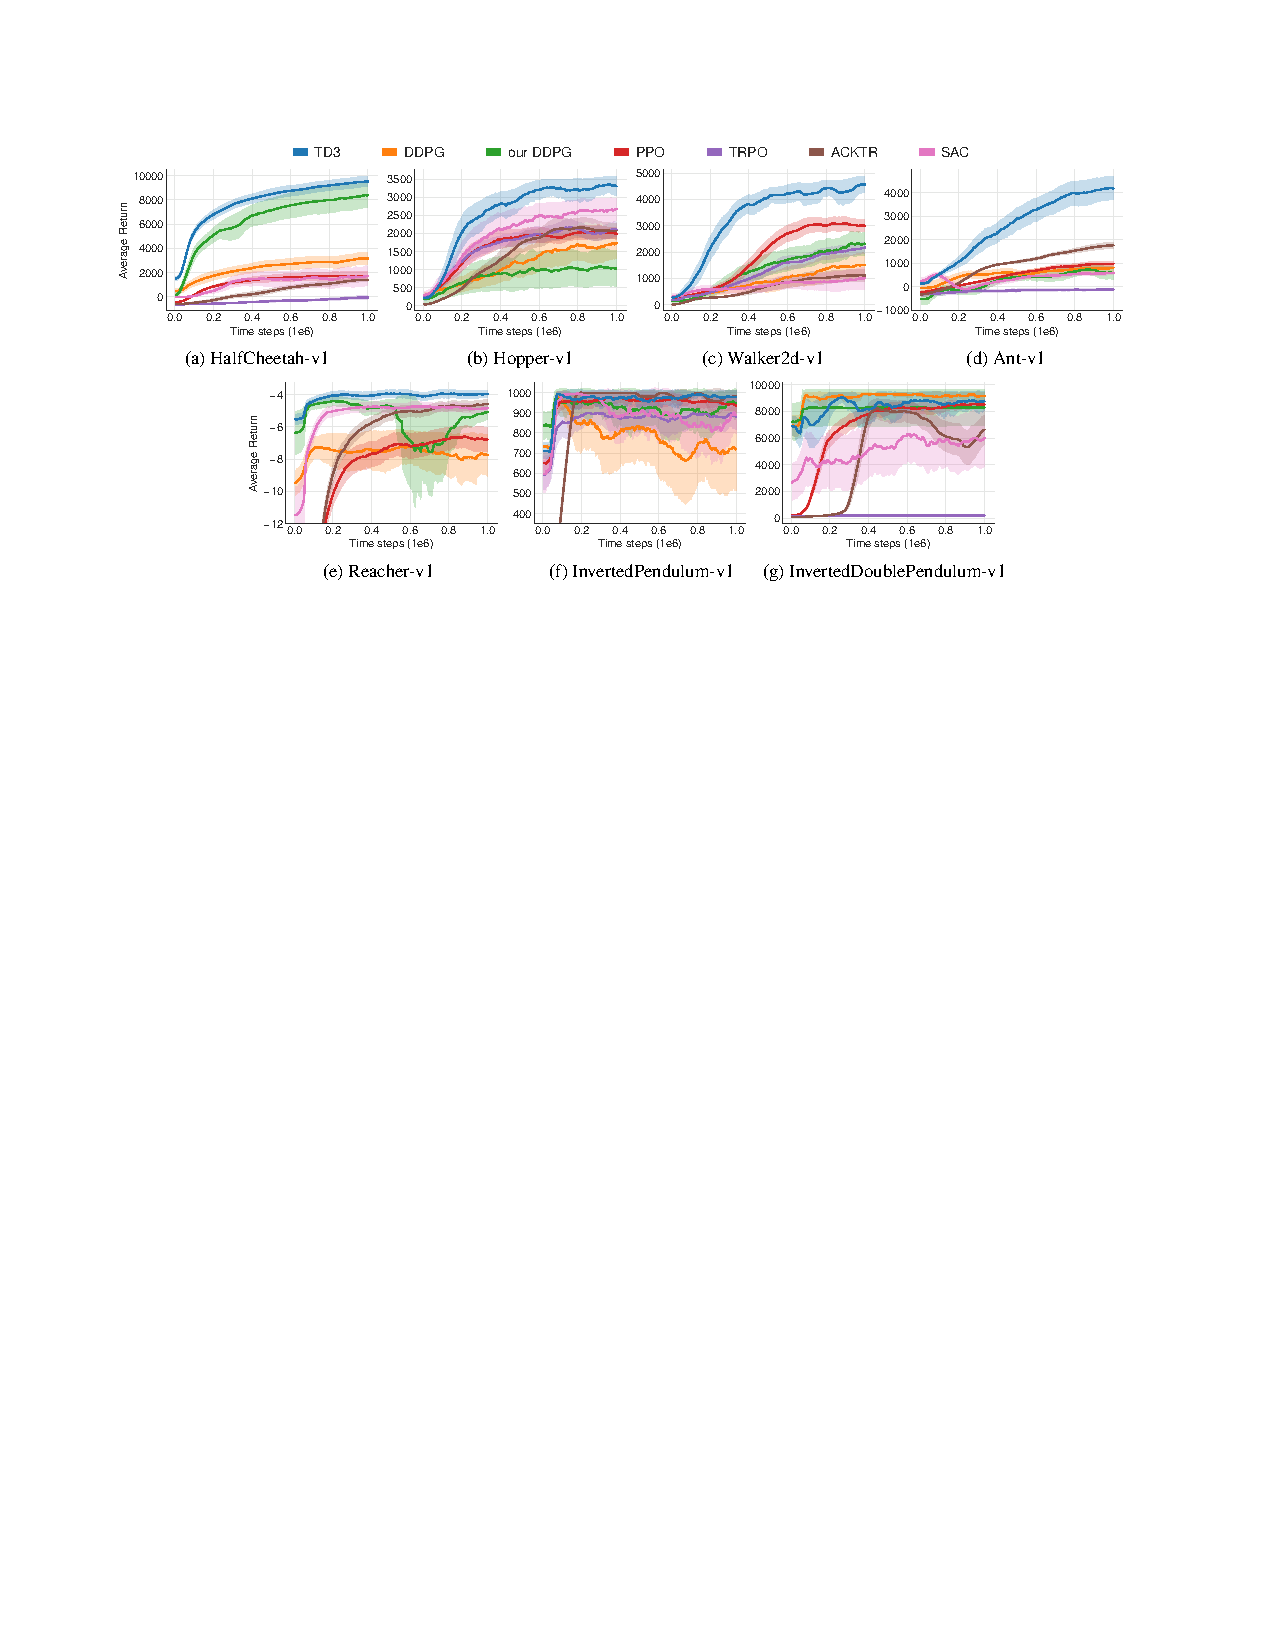
\includegraphics[height=5.25cm]{fig/lec13/Algo_Compare.pdf}
\caption{Learning curves for \href{https://gym.openai.com/envs/\#mujoco}{OpenAI Gym} continuous control tasks. The shaded region represents half a standard deviation of the average evaluation over ten trials (source: S. Fujimoto et al., \textit{Addressing Function Approximation Error in Actor-Critic Methods}, 2018).}
\label{fig:Algo_Compare}
\end{figure}
}	

%%%%%%%%%%%%%%%%%%%%%%%%%%%%%%%%%%%%%%%%%%%%%%%%%%%%%%%%%%%%%
%% Outlook: Other Contempororay Algorithms (1)%%
%%%%%%%%%%%%%%%%%%%%%%%%%%%%%%%%%%%%%%%%%%%%%%%%%%%%%%%%%%%%%
\frame{\frametitle{Algorithmic outlook: other contemporary model-free algorithms (1)}
The selection of algorithms appears endless:
\begin{itemize}
	\item DQN variants such as
	\begin{itemize}
		\item \href{https://arxiv.org/abs/1511.06581}{(Prioritized) dueling DQN}
		\item \href{https://arxiv.org/abs/1706.10295}{Noisy DQN}
		\item \href{https://arxiv.org/abs/1707.06887}{Distributional DQN}
	\end{itemize}\pause
	\item \href{https://ojs.aaai.org/index.php/AAAI/article/view/11796}{Rainbow} (combining multiple DQN extensions)\pause
	\item \href{https://arxiv.org/abs/1801.01290}{Soft actor-critic (SAC)}\pause
	\item \href{https://proceedings.neurips.cc/paper/2017/file/361440528766bbaaaa1901845cf4152b-Paper.pdf}{Actor critic using Kronecker-factored trust region (ACKTR)}\pause
	\item \href{http://proceedings.mlr.press/v48/mniha16.pdf}{Asynchronous advantage actor-critic (A3C)}
	\item ....
\end{itemize}
\vspace{0.5cm}\pause
Remarks: 
\begin{itemize}
	\item \hl{You have already learned the basic building blocks in order to make yourself familiar with any value-/policy-based model-free RL approach. \pause
	\item Use this knowledge! \pause
	\item Focus on primary scientific literature for self-studying and not on unreliable sources!} 
\end{itemize}
}

%%%%%%%%%%%%%%%%%%%%%%%%%%%%%%%%%%%%%%%%%%%%%%%%%%%%%%%%%%%%%
%% Outlook: Other Contempororay Algorithms (2)%%
%%%%%%%%%%%%%%%%%%%%%%%%%%%%%%%%%%%%%%%%%%%%%%%%%%%%%%%%%%%%%
\frame{\frametitle{Algorithmic outlook: other contemporary model-free algorithms (2)}
Algorithm collections with tutorial-style documentation:
\begin{itemize}
	\item \href{https://nervanasystems.github.io/coach/}{Intel Reinforcement Learning Coach}
	\item \href{https://spinningup.openai.com/en/latest/index.html}{OpenAI Spinning Up}
\end{itemize}\pause
\vspace{0.75cm}
Algorithm collections with decent application-oriented documentation:
\begin{itemize}
	\item \href{https://github.com/ray-project/ray}{RLlib (Ray)}
	\item \href{https://github.com/DLR-RM/stable-baselines3}{Stable Baselines3}
	\item \href{https://github.com/deepmind/acme}{Acme}
	\item \href{https://github.com/google/dopamine}{Google Dopamine}
	\item \href{https://github.com/tensorflow/agents}{TF-Agents}
	\item ...
\end{itemize}
}


%%%%%%%%%%%%%%%%%%%%%%%%%%%%%%%%%%%%%%%%%%%%%%%%%%%%%%%%%%%%%
%% Summary %%
%%%%%%%%%%%%%%%%%%%%%%%%%%%%%%%%%%%%%%%%%%%%%%%%%%%%%%%%%%%%%
\begin{frame}
\frametitle{Summary: what you've learned today}
\begin{itemize}
	\item Trust region policy optimization (TRPO) pursues monotonically increasing policy performance by limiting policy distribution changes.\pause
	\item This results in a nonlinear constrained optimization problem adding computational complexity (no simple policy gradients).\pause
	\item Proximal policy optimization (PPO) converts the TRPO idea into an unconstrained optimization problem by a modified objective. Likewise, the PPO's objective is to prevent erratic policy distribution changes. 
\end{itemize}
\end{frame}